\section{Introduction}
\label{sec:intro}

% Sources (paper-comp/CVCS-AI-Assisted-ID/): PAPER.md §1-§2; teaser
% figures/final/english/f_final_teaser_valid.sources.txt; test numbers results/csv_final/
% test_summary.csv, test_paired_deltas.csv; replicas results/csv_multiseed/ensemble_D.csv;
% curve results/csv_final/test_curve.csv and figures/final/english/f_final_curve.sources.txt.

\begin{figure}[t]
  \centering
  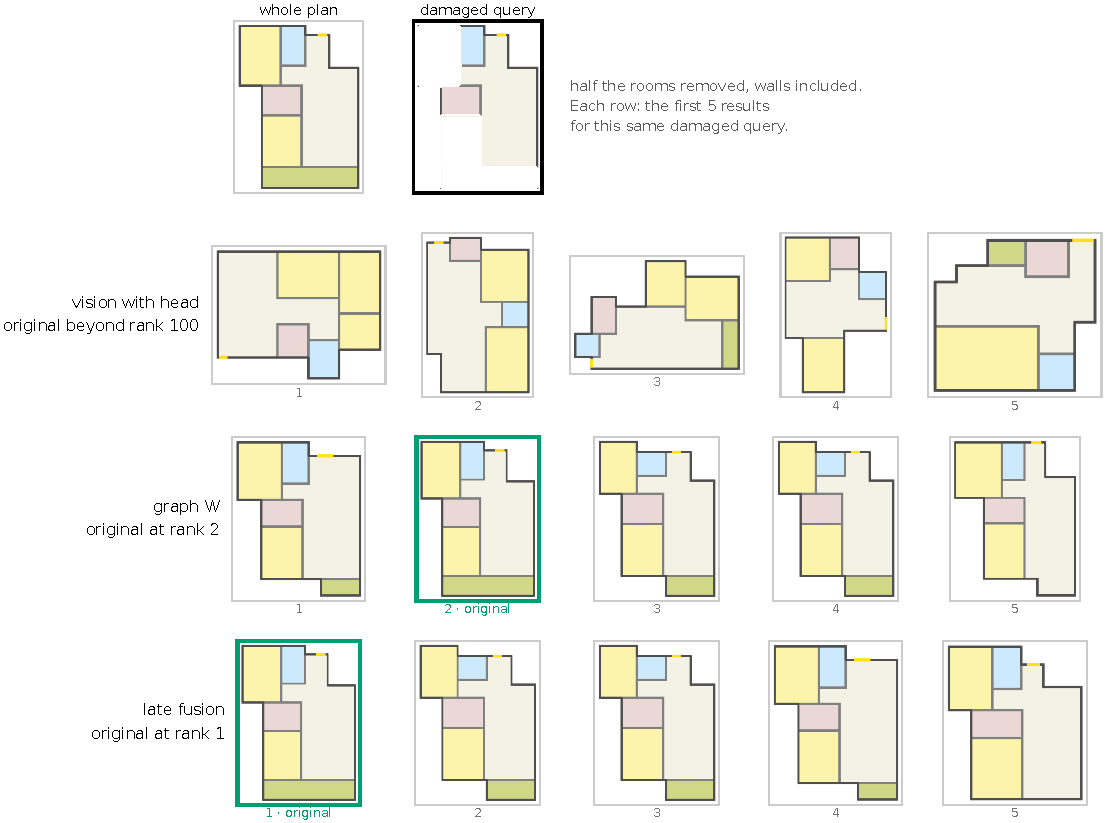
\includegraphics[width=\linewidth]{figures/english/f_final_teaser_valid.pdf}
  \caption{\textbf{Retrieving a plan from half of its rooms.}
  Top 5 of each system for one validation query; a frame marks the source.
  The single-damage vision head misses it, the graph ranks it second behind a near-identical plan, and the fusion ranks it first.
  The query is the first, alphabetically, of the 34 validation queries at this level where only the fusion ranks the source first.}
  \label{fig:teaser}
\end{figure}

% Stakes: architects search precedents from partial layouts.
Architects rarely start from a complete floor plan.
They sketch a few rooms, fix an outline or reuse a fragment of an existing plan, and then look for complete plans that contain it.
A retrieval system for this workflow must rank a large collection of plans from an \emph{incomplete} query and still find the plan the fragment came from.

% Problem gap: two structural limitations of current practice.
Two gaps separate current methods from this workflow.
First, floor-plan similarity methods learn and evaluate on complete plans: LayoutGMN~\cite{patil2021layoutgmn} and LayoutGKN~\cite{vanengelenburg2025layoutgkn} learn a structural similarity between complete RPLAN plans and score it with triplet accuracy or precision among their own top results.
Partial plans appear in floor-plan generation~\cite{hu2020graph2plan,zeng2026plancraft}, and we found no retrieval method that takes them as queries.
Second, a plan exists both as an image and as a graph of rooms, and fusing the two looks attractive because they fail in different ways: the image keeps the outline of a missing room, while a partial graph is the plausible complete graph of many smaller plans.
Yet any fusion of two models with partly independent errors gains accuracy; a fusion gain alone cannot tell whether the image adds information the graph lacks or merely acts as a second model.

% Key abstraction: ensemble controls and the complementarity gain.
We separate the two with \emph{ensemble controls}: we fuse the graph with a second model that holds the same information, either a second training of the same graph encoder or another graph encoder.
We call \emph{complementarity gain} (CG) the part of the vision--graph gain that the stronger control does not reach.
A positive CG means the image contributes information of its own.

% Design intuition.
FusePlan has two retrieval branches over the same gallery of 67{,}405 RPLAN plans~\cite{wu2019rplan} (\cref{fig:pipeline}).
The graph branch is a GATv2 encoder~\cite{brody2022gatv2} trained to map a plan with rooms removed onto the complete plan, with the checkpoint chosen on retrieval robustness.
The vision branch is a frozen PE-Spatial encoder~\cite{bolya2025perception} with whitening, optionally followed by a head trained on the same damages.
A late fusion with a single weight combines their cosine similarities.
We measure robustness as the self-recovery of the source plan when we remove rooms, a region or image patches, choose everything on validation and read the test split with the predictions written in advance.

% Results preview.
On the test split, the graph branch recovers the source with an AUC of 0.903, against 0.611 for LayoutGKN retrained on the same task.
Fusing it with the frozen image encoder adds $+0.013$, a gain that a second graph model matches; fusing it with a damage-trained vision head adds $+0.031$ (\cref{fig:teaser}), and over four replicas the damage-trained heads exceed both controls by $+0.012$ to $+0.022$.
The fusion gain follows an inverted U in the strength of the graph: it peaks at $+0.198$ when the two branches are equally strong, where even the frozen encoder passes both controls.

\noindent We make the following contributions:
\begin{itemize}
  \item \textbf{Graph branch for incomplete plans.} Training on damaged--complete pairs and selecting on robustness, after the same search over GCN, GraphSAGE and GATv2, brings self-recovery under room removal to $0.904\pm0.001$ on test, $0.29$ above a retrained LayoutGKN.
  \item \textbf{Ensemble controls and complementarity gain.} With a strong graph, a frozen image encoder adds no information beyond an ensemble effect, while damage-trained vision heads do; even then the control accounts for about half of the fusion gain, and the CG appears only where the graph has little left.
  \item \textbf{Relative strength.} Across 37 graphs, the fusion gain peaks when the branches are equally strong and shrinks near the ceiling, which reconciles a $+0.17$ gain in an earlier version of our pipeline with $+0.013$ here.
  \item \textbf{Protocol and negative results.} A self-recovery protocol with three damages, paired intervals, replicas and pre-registered test readings, and the failures that shaped it: a rendering artifact, a head that learns only the damage it sees, and a graph that collapses with symmetric pairs.
\end{itemize}
